% \documentclass[]{article}
% \usepackage{lmodern}
% \usepackage{amssymb,amsmath}
% \usepackage{ifxetex,ifluatex}
% \usepackage{fixltx2e} % provides \textsubscript
% \ifnum 0\ifxetex 1\fi\ifluatex 1\fi=0 % if pdftex
%   \usepackage[T1]{fontenc}
%   \usepackage[utf8]{inputenc}
% \else % if luatex or xelatex
%   \ifxetex
%     \usepackage{mathspec}
%     \usepackage{xltxtra,xunicode}
%   \else
%     \usepackage{fontspec}
%   \fi
%   \defaultfontfeatures{Mapping=tex-text,Scale=MatchLowercase}
%   \newcommand{\euro}{€}
% \fi
% % use upquote if available, for straight quotes in verbatim environments
% \IfFileExists{upquote.sty}{\usepackage{upquote}}{}
% % use microtype if available
% \IfFileExists{microtype.sty}{%
% \usepackage{microtype}
% \UseMicrotypeSet[protrusion]{basicmath} % disable protrusion for tt fonts
% }{}
% \usepackage[margin=1in]{geometry}
% \usepackage{longtable,booktabs}
% \usepackage{graphicx}
% \makeatletter
% \def\maxwidth{\ifdim\Gin@nat@width>\linewidth\linewidth\else\Gin@nat@width\fi}
% \def\maxheight{\ifdim\Gin@nat@height>\textheight\textheight\else\Gin@nat@height\fi}
% \makeatother
% % Scale images if necessary, so that they will not overflow the page
% % margins by default, and it is still possible to overwrite the defaults
% % using explicit options in \includegraphics[width, height, ...]{}
% \setkeys{Gin}{width=\maxwidth,height=\maxheight,keepaspectratio}
% \ifxetex
%   \usepackage[setpagesize=false, % page size defined by xetex
%               unicode=false, % unicode breaks when used with xetex
%               xetex]{hyperref}
% \else
%   \usepackage[unicode=true]{hyperref}
% \fi
% \hypersetup{breaklinks=true,
%             bookmarks=true,
%             pdfauthor={Rhian Davies},
%             pdftitle={Exploration},
%             colorlinks=true,
%             citecolor=blue,
%             urlcolor=blue,
%             linkcolor=magenta,
%             pdfborder={0 0 0}}
% \urlstyle{same}  % don't use monospace font for urls
% \setlength{\parindent}{0pt}
% \setlength{\parskip}{6pt plus 2pt minus 1pt}
% \setlength{\emergencystretch}{3em}  % prevent overfull lines
% \setcounter{secnumdepth}{0}

% %%% Use protect on footnotes to avoid problems with footnotes in titles
% \let\rmarkdownfootnote\footnote%
% \def\footnote{\protect\rmarkdownfootnote}

% %%% Change title format to be more compact
% \usepackage{titling}

% % Create subtitle command for use in maketitle
% \newcommand{\subtitle}[1]{
%   \posttitle{
%     \begin{center}\large#1\end{center}
%     }
% }

% \setlength{\droptitle}{-2em}
%   \title{Exploration}
%   \pretitle{\vspace{\droptitle}\centering\huge}
%   \posttitle{\par}
%   \author{Rhian Davies}
%   \preauthor{\centering\large\emph}
%   \postauthor{\par}
%   \date{}
%   \predate{}\postdate{}


% \begin{document}

% \maketitle


We shall split the features into customer features and quote features.

The customer features are Age of Driver, Age of Car, Expected Value of
Car, CC and policy duration. The three Value features are outcomes
relating to the customer features and such should be treated
differently.

\paragraph{Customer Features}\label{customer-features}

Of the 5 customer features, 4 of them are interval. The summaries for
these four variables are shown in table REF.

\begin{longtable}[c]{@{}lrrrrrr@{}}
\toprule
& Min & Max & Mean & Standard Deviation & Median &
Skewness\tabularnewline
\midrule
\endhead
Age\_of\_Driver & 18 & 81 & 46.03 & 13.00 & 44 & 0.52\tabularnewline
Age\_of\_Car & 0 & 31 & 10.90 & 5.25 & 11 & 0.40\tabularnewline
Expected\_Value\_of\_Car & 1000 & 99999 & 5319.51 & 4967.40 & 4000 &
3.60\tabularnewline
CC & 100 & 7000 & 1445.80 & 325.23 & 1390 & 2.40\tabularnewline
\bottomrule
\end{longtable}

The boxplots indicate the skewness and outliers in each feature.

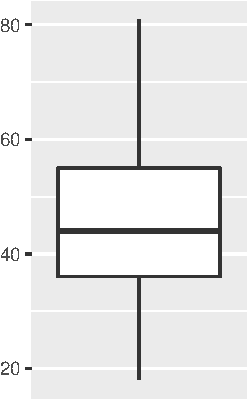
\includegraphics{exploration_files/figure-latex/dist_boxplots-1.pdf}
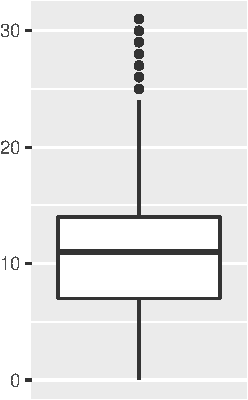
\includegraphics{exploration_files/figure-latex/dist_boxplots-2.pdf}
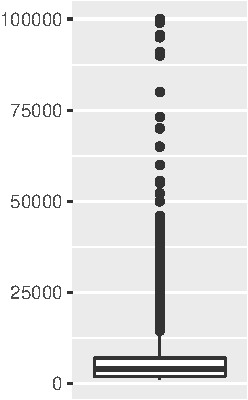
\includegraphics{exploration_files/figure-latex/dist_boxplots-3.pdf}
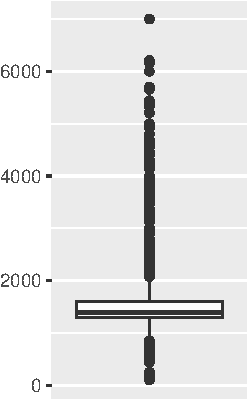
\includegraphics{exploration_files/figure-latex/dist_boxplots-4.pdf}

The final customer feature is the policy duration. The customer can
select if they are interested in a 6 or 12 month policy. Policy duration
takes only two values, 6 months or 12 months. We shall treat this as a
symmetric binary variable ``isthepolicy6months''. There are roughly an
equal amount of both types of policies. In the data set there are 224578
6 months policies and 240537 12 month policies.

\paragraph{Quote features}\label{quote-features}

\paragraph{Streaming aspect}\label{streaming-aspect}

As stated above, the data is recieved as a stream, and thus we have
timestamped data. It is worth examining how the volume of data evolves
over the stream. We have approximately 3 months of data.

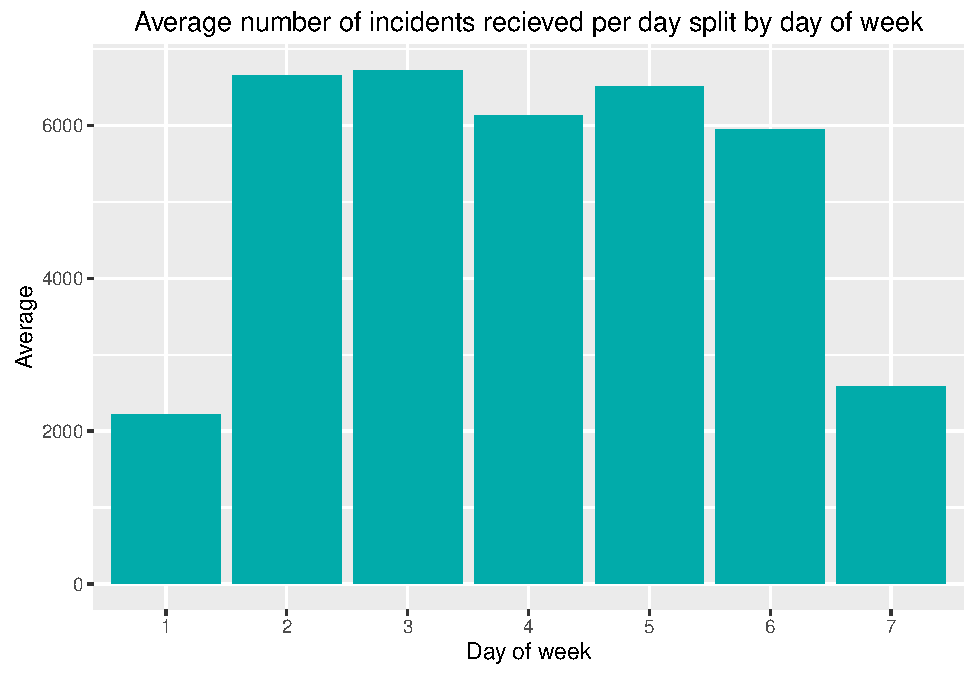
\includegraphics{exploration_files/figure-latex/observations_per_day-1.pdf}

We can see in Figure REF that more requests are recieved on week days
than on weekends as might be expected. We can also observe the
distribution over time of day.

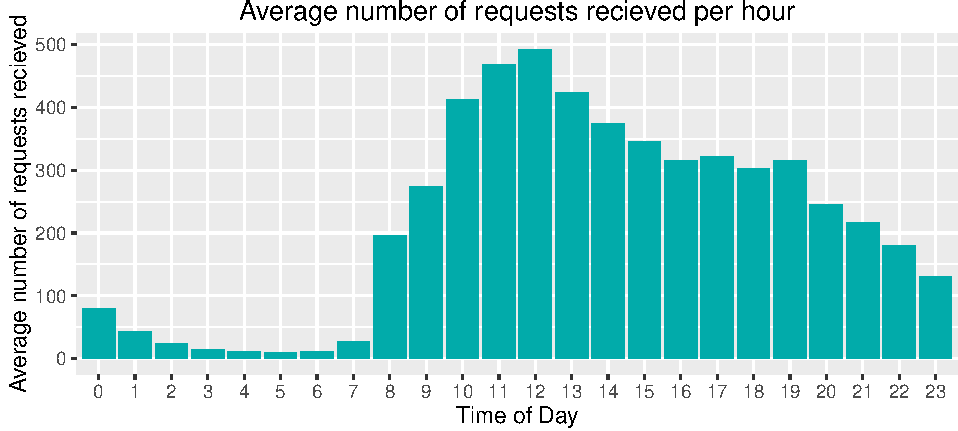
\includegraphics{exploration_files/figure-latex/distribution_of_requests-1.pdf}

This is what we would expect to see with peak number of requests
occuring beteen 10am and 7pm.

Finally we can look if there exists any sort of seasonal trend within
the volume of calls.

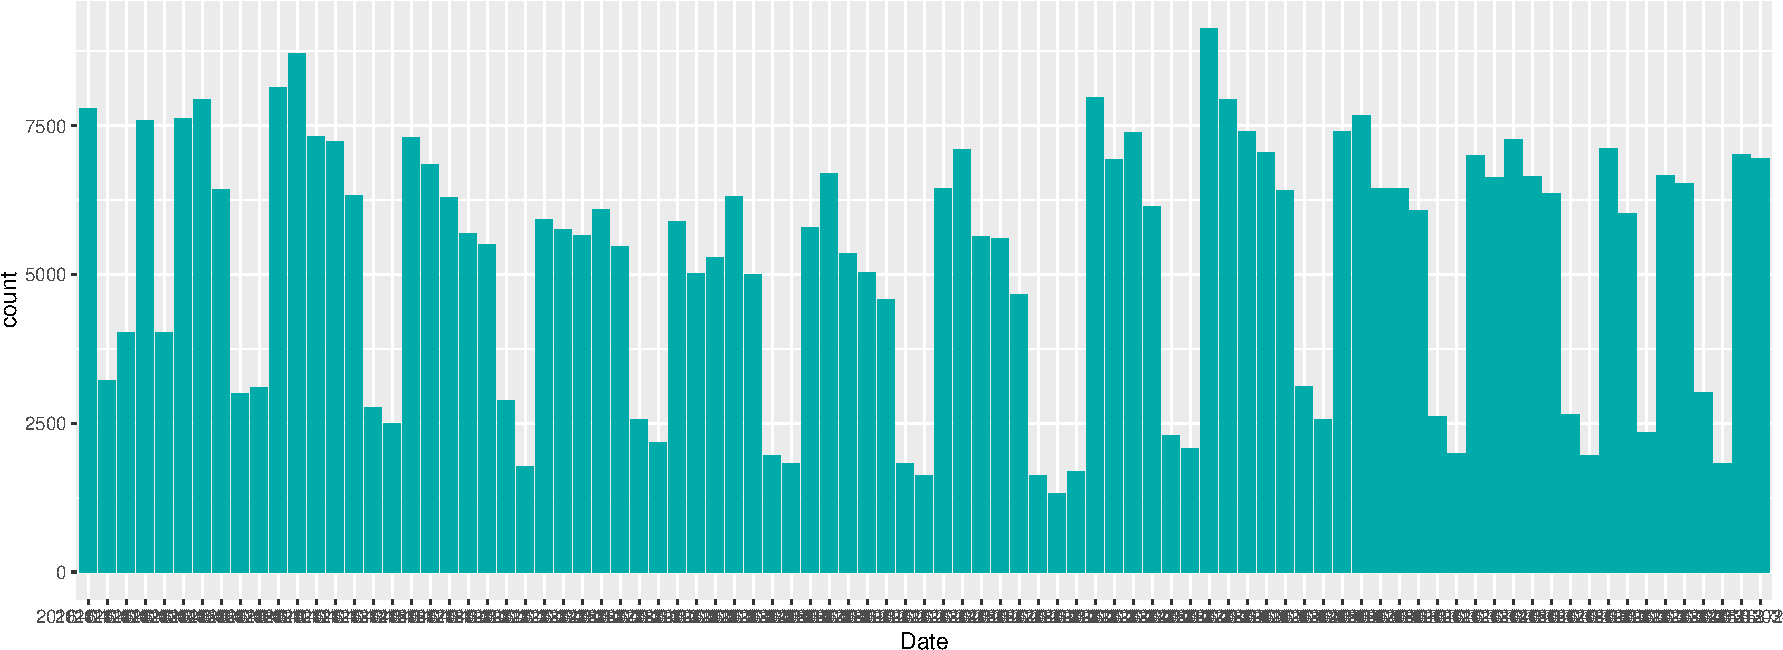
\includegraphics{exploration_files/figure-latex/total_requests_policy_duration_week-1.pdf}

%\end{document}
